\section{实验评估}
\label{sec:experiments_zh}

\subsection{基准配置与执行核验}
\label{sec:setup_zh}

表~\ref{tab:measured_design}所列基准从观察到的价格向上游追溯。日内轨迹（RQ1）在匹配随机流下度量成交频率和双边盘口覆盖率，区分何时有新成交、何时有双边报价可计算价差。共同父世界分支（RQ2）追踪同一感染事件后的社会状态，并检验行为机制与监管制度如何改变委托和成交。固定观察与调度核对（RQ3）进一步考察不同后端如何由观察生成意图，以及哪些计划请求有机会收到公开公告。规则世界的运行剖面度量保存和核验状态历史所需的开销。

\begin{table*}[t]
  \centering\small
  \caption{\tr{实测基准及离线调度核对的配置。长周期参考配置见附录~\ref{app:benchmark_details_zh}。}{Settings for the Measured Benchmarks and Offline Schedule Audit. Appendix~\ref{app:benchmark_details} gives the prospective long-horizon configuration.}}
  \label{tab:measured_design}
  \begin{tabularx}{\textwidth}{@{}p{0.24\textwidth} p{0.28\textwidth} X@{}}
    \toprule
    \tr{评估任务}{Evaluation} & \tr{执行配置}{Settings} & \tr{比较单位}{Unit of comparison} \\
    \midrule
    \tr{日内交易活动（RQ1）}{Intraday activity (RQ1)} &
    $N=100$, $T=T_{\rm day}=100$, $p_{\rm act}=0.05$ &
    \tr{三个匹配种子，各比较三种规则策略。}{Three matched seeds, each shared by three rule policies.} \\
    \tr{共同父世界分支（RQ2）}{Shared-parent branches (RQ2)} &
    $N=20$, $T_{\rm day}=4$, $p_{\rm act}=1$, \tr{27 步事件窗}{27 event steps} &
    \tr{一个父世界，十一条分支。}{Eleven branches from one parent world.} \\
    \tr{固定观察（RQ3）}{Fixed observations (RQ3)} &
    \tr{九类画像 $\times$ 三类对比 $\times$ 两个状态}{Nine archetypes $\times$ three contrasts $\times$ two states} &
    \tr{54 次真实 LLM 请求，构成 27 对比较。}{54 live LLM requests, organized into 27 pairs.} \\
    \tr{离线调度核对（RQ3）}{Offline scheduling (RQ3)} &
    $N=100$, $p_{\rm act}=0.05$, $k=10$, $T_{\rm slow}=10$ &
    \tr{20 个固定种子在公告发布步的计划资格。}{Scheduled eligibility at announcement release across 20 fixed seeds.} \\
    \tr{规则运行剖面（RQ3）}{Rule profiles (RQ3)} &
    \tr{同一平台 $N=100$、$T=100,200$；另一平台 $N=1{,}000$、$T=12$}{Same host $N=100$, $T=100,200$; second host $N=1{,}000$, $T=12$} &
    \tr{Mac 各期限一次完整剖面；ASUS 保存 12 步、终期剖面未完成。}{One complete Mac profile per horizon. The ASUS run saved 12 steps and stopped during final profiling.} \\
    \bottomrule
  \end{tabularx}
\end{table*}


三种规则策略使用种子 932201--932203。全部 900 个提交步的现金、股份与税费残差均为零，同平台只读恢复所得终态哈希与九条轨迹各自的归档一致（表~\ref{tab:invariants}）。跨策略比较以配对种子为单位。

\subsection{市场活动与盘口覆盖率（RQ1）}
\label{sec:exp:rq1_zh}

同一种子下的各策略共用活跃掩码、对数正态报价扰动、资源约束及撮合规则。零智能主体以对称概率买入或卖出，也可以观望~\cite{gode1993allocative}。同质线性价值基线保留建仓成本与近期高点，采用线性估值与固定风险容忍度 0.5，其委托策略不包含社会反馈和动态损失反馈。

\begin{figure*}[t]
 \centering
 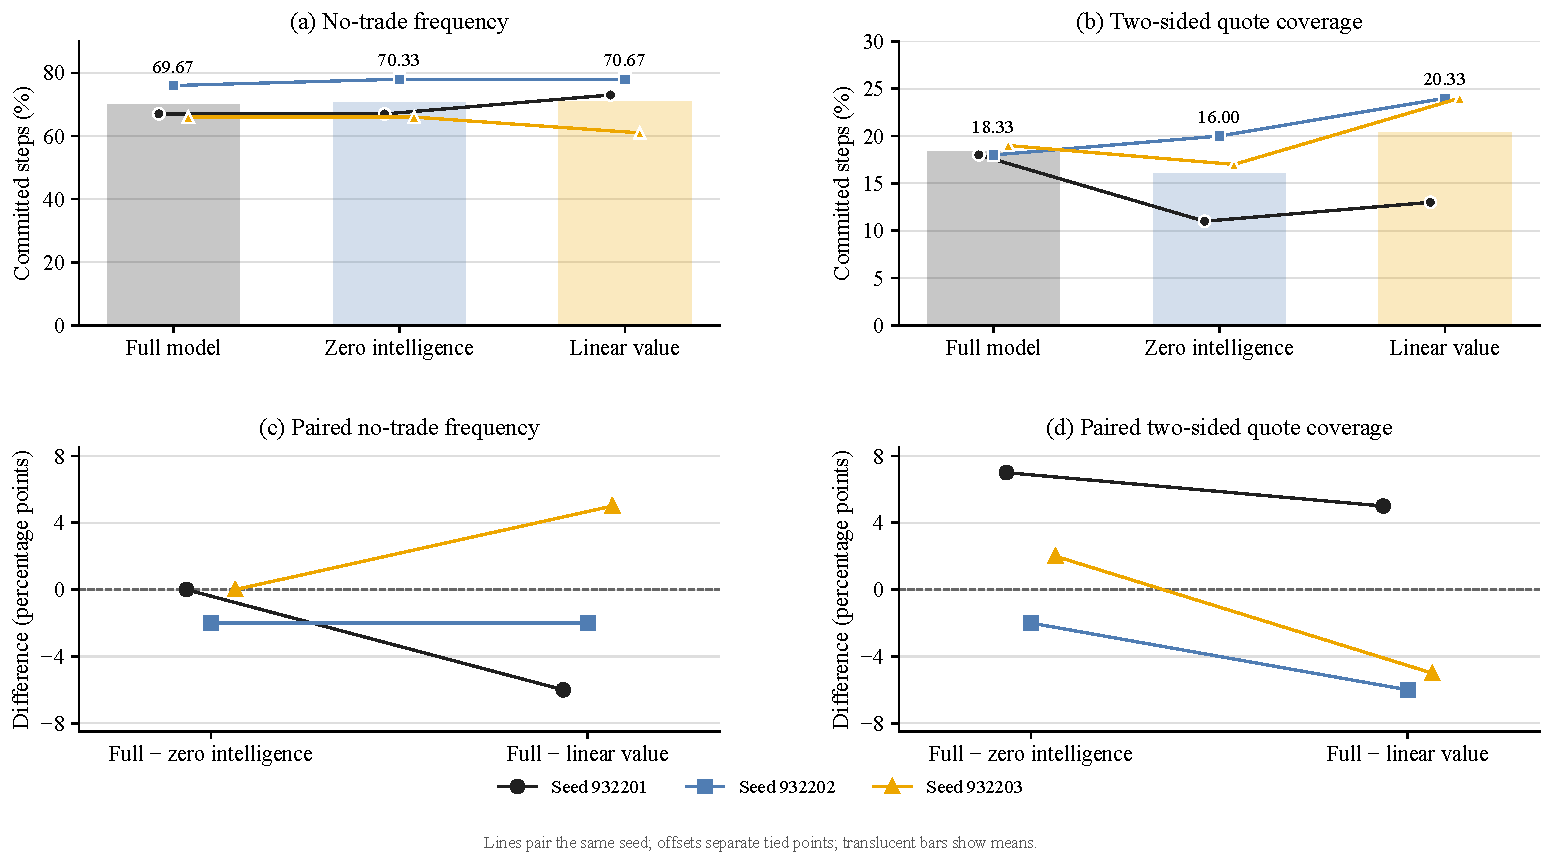
\includegraphics[width=0.96\textwidth]{figures/fig2_rq1_stylized_facts.pdf}
 \caption{九条规则轨迹的日内市场活动。上排为无成交步与双边盘口覆盖率，下排为同一种子下完整模型减去各基线的差值，单位为百分点。上排柱为跨种子均值，点线连接同一种子下的各策略结果。同位置的点略作横移以便辨认。}
 \Description{九条轨迹的市场活动、双边盘口覆盖率与种子内配对差。}
 \label{fig:rq1_zh}
\end{figure*}

\paragraph{盘口覆盖率随配对种子变化。}
在活跃率 0.05、挂单单步有效的配置下，61\%--78\% 的步无成交，11\%--24\% 的步同时存在买卖报价。完整模型平均有 69.67\% 的步无成交，双边报价覆盖率为 18.33\%。零智能基线相应为 70.33\% 和 16.00\%，线性价值基线为 70.67\% 和 20.33\%。完整模型的覆盖率相对零智能基线的种子内差值为 $+7,-2,+2$ 个百分点，相对线性价值基线为 $+5,-6,-5$ 个百分点，覆盖率排序随种子变化（图~\ref{fig:rq1_zh}、表~\ref{tab:rq1_results}）。

报价价差 $10^4(P^{\rm ask}-P^{\rm bid})/P^{\rm mid}$ 的样本为买卖队列同时存在的可交易步。联合报告覆盖率可以明确条件价差的统计分母。每条实测轨迹覆盖一个模型交易日。多日评价方案基于日对数收益率 $r_d=\log(P_d/P_{d-1})$，考察超额峰度、收益率与绝对收益率的自相关，以及成交量与 $|r_d|$ 的相关性~\cite{cont2001empirical}（附录~\ref{app:benchmark_details_zh}）。

\subsection{跨尺度反馈与政策反事实（RQ2）}
\label{sec:exp:rq2_zh}

\begin{figure*}[t]
 \centering
 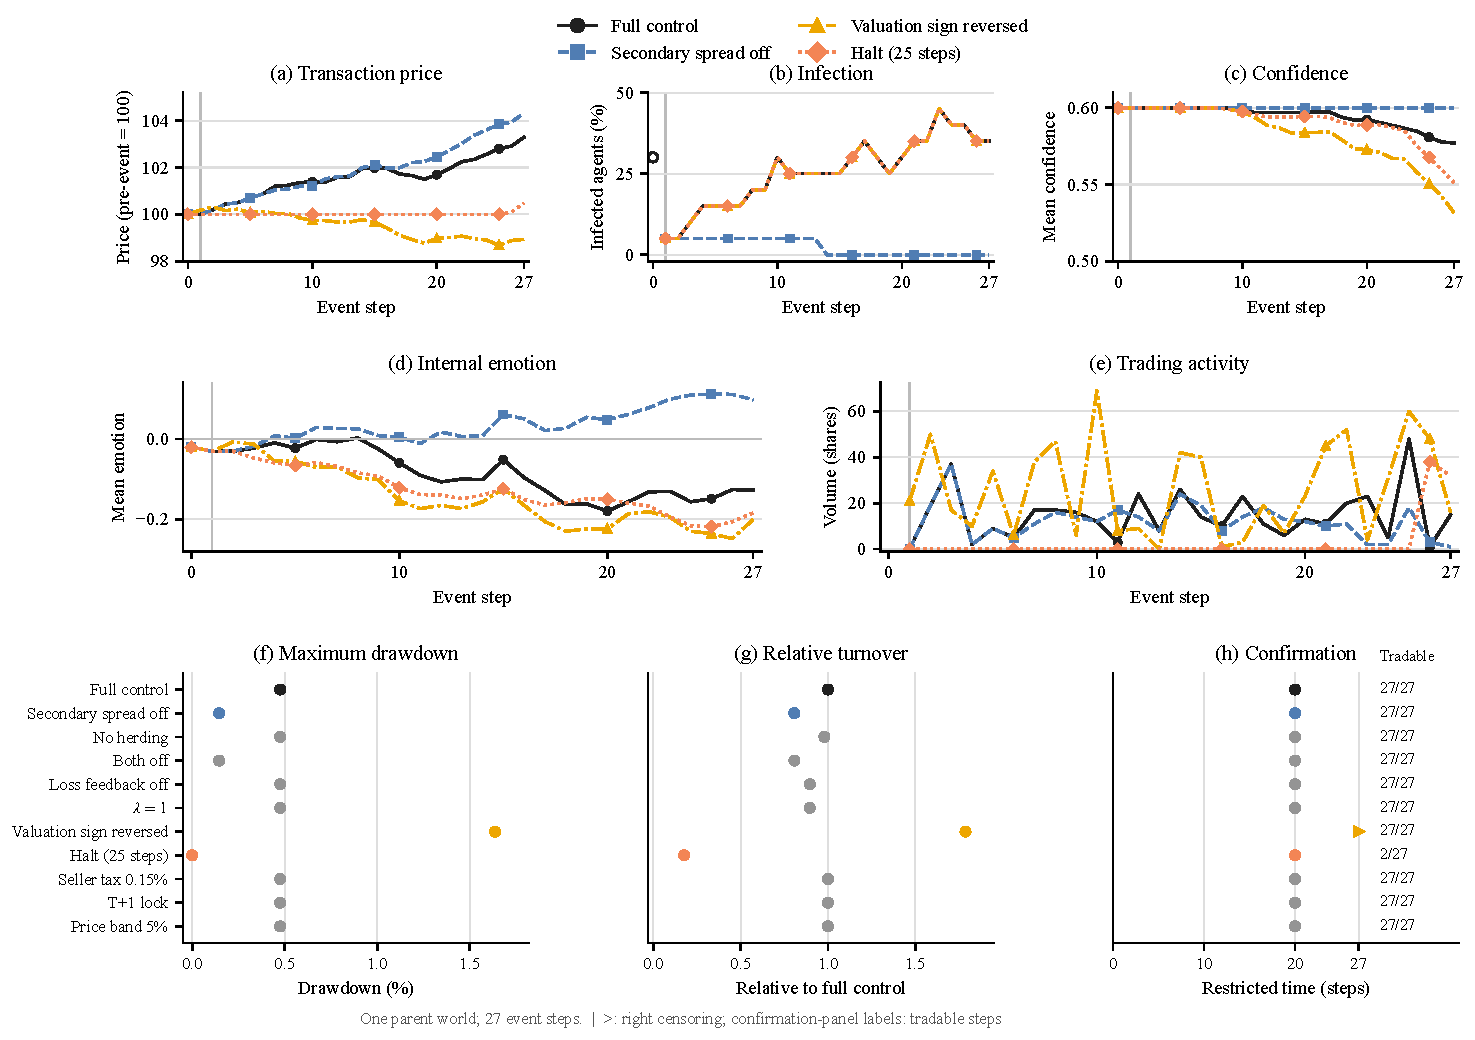
\includegraphics[width=\textwidth]{figures/fig3_rq2_mechanisms_policy.pdf}
 \caption{同一父世界的社会、行为和市场响应。时序面板按同一事件时钟对齐感染比例、模型内部信心与情绪的均值、价格指数及成交股数。图 (b) 的空心点标记事前检查点（20 人中有 6 人感染）。共同事件在 $u=1$ 将全员重置为易感态，再注入一例感染（20 人中有 1 人感染）。下排对照全部十一条分支，箭头标记 $u=27$ 时的右删失。}
 \Description{五组共用事件时间的状态及交易时序，以及三个分支结果面板。}
 \label{fig:rq2_zh}
\end{figure*}

\paragraph{共同检查点分支。}
各分支从种子 933001 的第 5 次提交开始，包含 20 名投资者，每个交易日 4 步，事件窗内每步所有主体均活跃。共同检查点 $u=0$ 已有 6 人处于感染态。在 $u=1$（仿真步 6），共同事件先将全员重置为易感态，再感染一名投资者。因此，事前的 30\% 与首个事件提交步的 5\% 分别对应这次共同重置前后的状态。各分支共用随机流并演化 27 个事件步。图~\ref{fig:rq2_zh}对齐每次提交的感染比例、平均信心与情绪、最新成交价及成交股数。

最大回撤为价格从运行峰值的最大相对跌幅，峰值由事前价格初始化。相对换手率为各分支成交股数除以完整对照的成交股数。价格确认记录首次全局谷底后连续 20 步价格达到事前价格 98\% 时的事件步，谷底可位于 $u=0$。窗口结束时未确认的分支按右删失记录（表~\ref{tab:rq2_results}）。

\paragraph{社会状态与市场响应。}
完整对照的感染率在 $u=23$ 达到 45\%（图~\ref{fig:rq2_zh}b）。平均信心从 $u=10$ 开始走低，窗口结束时为 0.577。平均内部情绪在 $u=20$ 降至 $-0.180$（图~\ref{fig:rq2_zh}c--d）。阻断二次传染后，感染限于初始的一名投资者，到 $u=14$ 清零。该分支的平均信心维持在约 0.600，平均情绪在 $u=25$ 达到 $+0.112$。关闭二次传染也使成交量从 395 股降至 319 股（图~\ref{fig:rq2_zh}e），末步价格指数从 103.28 升至 104.31（图~\ref{fig:rq2_zh}a）。最大回撤从 0.4754\% 降至 0.1453\%，下降 0.3301 个百分点，相对降幅为 69.4\%。

关闭信心依赖从众后，感染峰值仍为 45\%。两条价格路径直到 $u=22$ 都相同，包括决定最大回撤的 $u=15$ 局部峰值和 $u=19$ 谷值，因此两条分支的最大回撤同为 0.4754\%。谷值当步的成交量已相差 1 股，事件窗总成交量从 395 股降至 387 股，相对换手率为 0.9797。令 $Y$ 为最大回撤，两项二元下标分别表示是否启用传染和从众。该父世界中四分支交互项 $Y_{11}-Y_{10}-Y_{01}+Y_{00}$ 为零。

\paragraph{回顾性估值的方向改变价格响应。}
共同事件改变社会状态，价格随其后的实际委托和成交更新。在式~\eqref{eq:aggregate_v_zh}中，价格高于回顾性参考点时，该项对估值的贡献为正。在其他输入固定时，它提高买入倾向，实际委托还取决于其他参考点、情绪及风险容忍度。反转回顾性偏差的符号后，末价较事前低 1.07\%，最大回撤升至 1.6372\%，相对换手率为 1.7873。设 $\lambda=1$ 的分支与进一步移除动态损失反馈的分支均录得 0.4759\% 的回撤及 0.8962 的相对换手率。

\paragraph{交易制度作用于委托与结算的不同环节。}
停牌 25 步后，27 步事件窗内有 2 步可交易，相对换手率为 0.1772，回撤为零。停牌开始时撤去挂单，随后 25 步无成交并沿用上一笔成交价。同期感染率峰值达 45\%，平均内部情绪在 $u=25$ 降至 $-0.218$。$u=26$ 恢复撮合后成交 38 股（图~\ref{fig:rq2_zh}a--e）。其余三个监管分支均保留 27 个可交易步，与对照的 87 笔成交完全相同。5\% 价带分支的委托价与成交价相对各交易日锚价最大偏离为 1.092\%。$T+1$ 锁定股份峰值为 72 股，归档的卖单与成交均未改变。0.15\% 卖方税直接影响结算扣款，在给定状态下式~\eqref{eq:order_quantity_zh}的股数计算保持不变。本事件窗成交相同，卖方税费收入由 20.286250 元增至 60.858750 元。

\paragraph{价格确认的下限反映了短窗口径。}
十个分支的首次谷底位于事前，均在最早可能的第 20 步达到确认条件。停牌分支在持续沿用上一笔成交价时达到该条件。反转估值分支第 25 步触底，之后只有两步，因而在第 27 步右删失。本次比较中所有价格均高于事前的 98\%。此处价格确认反映谷底后的观测步数，需要结合可交易步及换手率解释。

\subsection{决策接口与计算开销（RQ3）}
\label{sec:exp:rq3_zh}

\begin{figure*}[t]
 \centering
 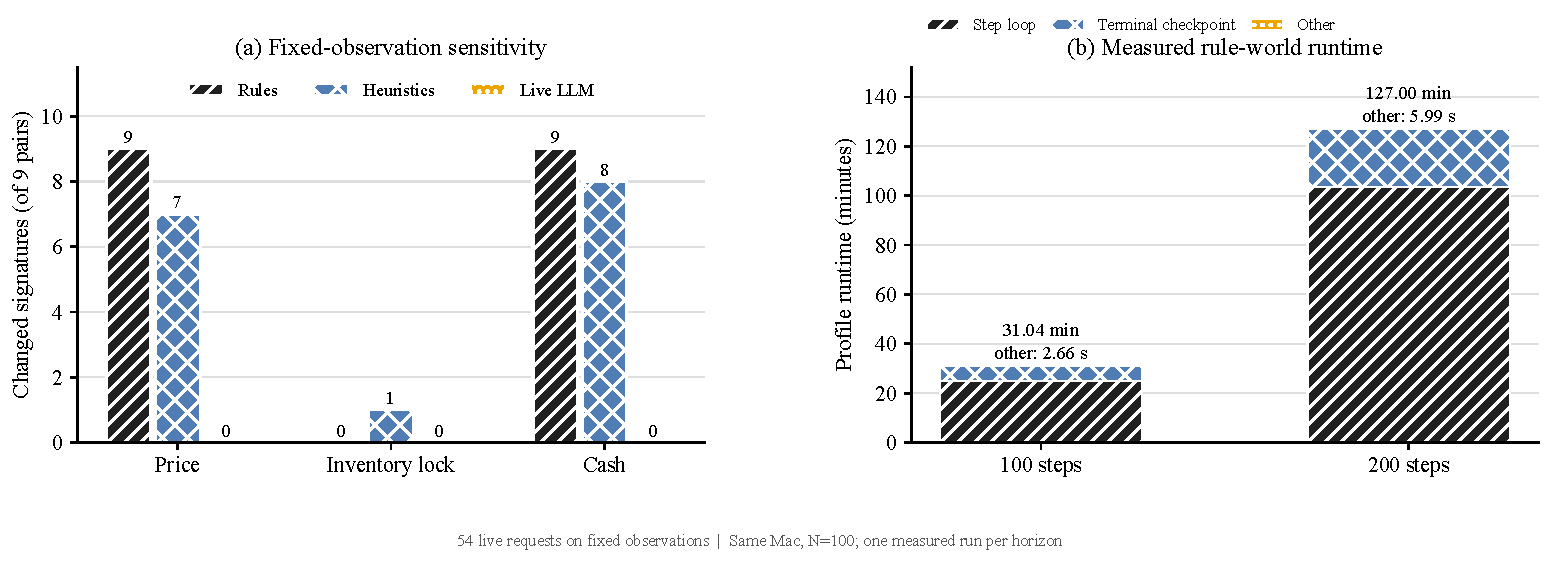
\includegraphics[width=\textwidth]{figures/fig4_rq3_cognition_cost.pdf}
 \caption{固定观察响应与规则世界运行剖面。响应面板给出每类九对观察中的经济动作签名变化数。运行面板拆分同一平台上两次 $N=100$ 规则运行的持久化步循环、终态检查点及其余时间。}
 \Description{三种状态对比的动作签名变化次数与两种仿真期限的分阶段耗时。}
 \label{fig:rq3_zh}
\end{figure*}

\paragraph{固定观察基准检验决策契约。}
九类画像各有价格、锁定股份与现金三种对比，每种对比包含两个状态。中性措辞下共形成 54 个请求单元、45 个不同的构造观察和 27 对比较。采样温度设为零，输出上限为 2,048 tokens。请求配置与归档的 OpenAI API 响应均以 \texttt{gpt-6-luna} 为模型别名。

经济动作签名由方向、带符号股数和限价组成。数值规则在 18/27 对、画像启发式在 16/27 对、LLM 在 0/27 对中改变签名（图~\ref{fig:rq3_zh}a、表~\ref{tab:pilot}）。数值规则输出 45 次买入、9 次观望。发给 LLM 的构造观察同时包含当期状态，以及私有 \texttt{behavior} 字段中保留的模板行为轨迹。54 份请求中，这两份记录的风险和参考价均存在差异。54 份响应均为 \texttt{HOLD}，并通过模式、协议身份、证据 ID 与资源可行性检查。证据检查验证引用 ID 互不重复且属于当次观察的可见集合。签名对比刻画了各后端在这组输入下的响应。要识别字段差异本身的作用，需加入状态与轨迹对齐的对照。

\paragraph{不同画像的委托变化。}
数值规则的价格对比在九类画像中均使带符号股数变化 $-2$ 股，现金对比均变化 $-12$ 股（图~\ref{fig:persona_deltas_zh}）。画像启发式在价格对比中使套利者和平准资金的带符号股数分别变化 $-102$ 股与 $-63$ 股。锁仓对比中，保险机构由卖出 10 股改为 \texttt{HOLD}。在另一组价格对比中，该画像的带符号股数保持不变，限价上移 1,002 个报价档位，对应图中的 $\dagger$。

\begin{figure*}[t]
 \centering
 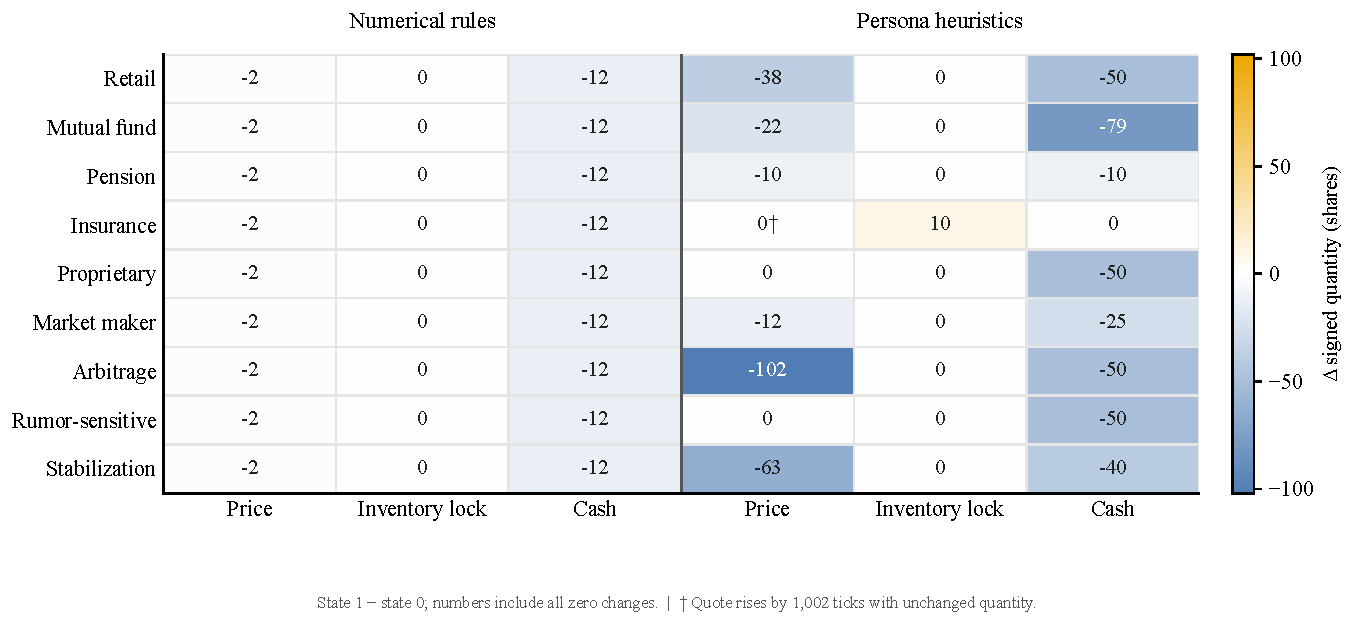
\includegraphics[width=0.96\textwidth]{figures/archetype_order_response.pdf}
 \caption{九类画像的带符号委托量变化。各单元为相应后端和对比下扰动状态减去基准状态的委托股数。买入记正，卖出记负，观望记零。符号 $\dagger$ 标记股数不变而限价变化的单元。}
 \Description{九类画像在数值规则和画像启发式各三种扰动下的带符号委托量变化。}
 \label{fig:persona_deltas_zh}
\end{figure*}

\paragraph{推理开销与公告的计划曝光机会。}
真实请求批次在 69.597 秒内消耗 119,637 个输入 tokens 和 9,306 个输出 tokens，单请求延迟中位数为 2.297 秒。按归档用量和冻结费率核算，成本上界为 0.03456225 美元（表~\ref{tab:rq3_results}）。独立的离线核对在公告发布步求取激活掩码与请求计划的交集。20 个固定种子的公告均落在周期请求步。全量调度共安排 101 次符合资格的请求，周期慢组在 10 个种子中各安排一次。其余 10 个种子在公告发布时均无活跃的慢组主体（图~\ref{fig:schedule_exposure_zh}右图）。式~\eqref{eq:cost_ratio_zh}给出全程的期望请求比例，发布步的计数则显示同一调度如何影响模型接收这次公告的机会。

\paragraph{累计历史的归档处理带来随期限增长的开销。}
在 Apple M5（24 GiB）上，相同种子、100 主体的规则世界由 100 步延长至 200 步时，剖面总耗时由 1,862.397 秒增至 7,619.767 秒，为原来的 4.091 倍。进程内存峰值由 1.239 GiB 增至 2.486 GiB。终态检查点包含已持久化增量链的重建，分别耗时 364.780 秒与 1,394.507 秒。执行、提交、持久化发布与终态检查点合计占两次总耗时的 89.9\% 和 91.0\%，决策阶段分别耗时 2.895 秒和 5.789 秒。

当前归档实现反复验证、复制并哈希累积的决策、回执和账本记录。固定种群且历史规模随 $t$ 线性增长时，每步一次全历史扫描产生 $\sum_{t=1}^{T}\mathcal{O}(t)=\mathcal{O}(T^2)$ 的累计访问成本。该项描述累积历史处理，图~\ref{fig:rq3_zh}记录完整运行器的两次实测。AMD Ryzen AI 7 H 350 平台的千主体规则运行保存了全部 12 步，采样内存峰值为 1.692 GiB，控制器在最终剖面阶段终止。同一个 100 主体、12 步世界的三组配对计时中，标量化严格校验使总用时下降 1.52\%--3.08\%（图~\ref{fig:timing_supp_zh}）。
